% mnras_template.tex
%
% LaTeX template for creating an MNRAS paper
%
% v3.0 released 14 May 2015
% (version numbers match those of mnras.cls)
%
% Copyright (C) Royal Astronomical Society 2015
% Authors:
% Keith T. Smith (Royal Astronomical Society)

% Change log
%
% v3.0 May 2015
%    Renamed to match the new package name
%    Version number matches mnras.cls
%    A few minor tweaks to wording
% v1.0 September 2013
%    Beta testing only - never publicly released
%    First version: a simple (ish) template for creating an MNRAS paper

%%%%%%%%%%%%%%%%%%%%%%%%%%%%%%%%%%%%%%%%%%%%%%%%%%
% Basic setup. Most papers should leave these options alone.
\documentclass[fleqn,usenatbib]{mnras}  % a4paper,

% MNRAS is set in Times font. If you don't have this installed (most LaTeX
% installations will be fine) or prefer the old Computer Modern fonts, comment
% out the following line
%\usepackage{newtxtext,newtxmath}
\usepackage{txfonts}
% Depending on your LaTeX fonts installation, you might get better results with one of these:
%\usepackage{mathptmx}
%\usepackage{txfonts}


% Use vector fonts, so it zooms properly in on-screen viewing software
% Don't change these lines unless you know what you are doing
\usepackage[T1]{fontenc}
\usepackage{ae,aecompl}
\usepackage{slashbox}

%%%%% AUTHORS - PLACE YOUR OWN PACKAGES HERE %%%%%

% Only include extra packages if you really need them. Common packages are:
\usepackage{graphicx}	% Including figure files
\usepackage{amsmath}	% Advanced maths commands
\usepackage{amssymb}	% Extra maths symbols

%%%%%%%%%%%%%%%%%%%%%%%%%%%%%%%%%%%%%%%%%%%%%%%%%%

%%%%% AUTHORS - PLACE YOUR OWN COMMANDS HERE %%%%%

% Please keep new commands to a minimum, and use \newcommand not \def to avoid
% overwriting existing commands. Example:
%\newcommand{\pcm}{\,cm$^{-2}$}	% per cm-squared

%%%%%%%%%%%%%%%%%%%%%%%%%%%%%%%%%%%%%%%%%%%%%%%%%%

%%%%%%%%%%%%%%%%%%% TITLE PAGE %%%%%%%%%%%%%%%%%%%

% Title of the paper, and the short title which is used in the headers.
% Keep the title short and informative.
\title[SDSS Quasars]{SDSS Stripe 82 : quasar variability from forced photometry}

% The list of authors, and the short list which is used in the headers.
% If you need two or more lines of authors, add an extra line using \newauthor
\author[K. Suberlak et al.]{
Krzysztof Suberlak,$^{1}$\thanks{E-mail: suberlak@uw.edu}
\v{Z}eljko Ivezi\'c, $^{1}$
Yusra AlSayyad,$^{1}$ 
\\
% List of institutions
$^{1}$Department of Astronomy, University of Washington, Seattle, WA, United States\\
}

% These dates will be filled out by the publisher
\date{Accepted XXX. Received YYY; in original form ZZZ}

% Enter the current year, for the copyright statements etc.
\pubyear{2015}

% Don't change these lines
\begin{document}
\label{firstpage}
\pagerange{\pageref{firstpage}--\pageref{lastpage}}
\maketitle

% Abstract of the paper
\begin{abstract}

\end{abstract}


%%%%%%%%%%%%%%%%%%%%%%%%%%%%%%%%%%%%%%%%%%%%%%%%%%

%%%%%%%%%%%%%%%%% BODY OF PAPER %%%%%%%%%%%%%%%%%%

\section{Introduction}
\label{sec:intro}


\section{Data Analysis}
\label{sec:data}

We use data from all SDSS runs up to an including run 7202 (Data Release 7), including all 6 SDSS camera columns. 

All epochs (individual images) were background-subtracted, and then scaled from the Digital Unit counts to fluxes by comparing standard objects against the Ivezic+2007 catalog  (similar to  Jiang+2014).   

The data were coadded, and all objects detected in the i-band coadds were assigned a deepSourceId (== objectId). For star-galaxy separation, the entire clump was considered as one parent source (with single ParentSourceId). For an object which is a parent (eg. a galaxy), ParentSourceId is null.  This amounts to $~40$ milion  i-band detections down to $3 \, \sigma$.  $8$ million of those are brighter than $23^{rd}$ mag. Thus the total number of photometric measurements is : ($40$  million i-band detections) x ($80$ epochs ) x ($5$ filters) = $~16$ billion measurements, including   ($8$ million i-band detections i < 23) x ($80$ epochs) x ($5$ filters ) = $~3$ billion measurements brighter than $23^{rd}$ mag.

Forced photometry was performed in u,g,r,i,z  on the individual epoch images (NOT difference imaging),  in locations specified by i-band coadds. (DIFFERENCE imaging is when photometry is done on  coadd - individual-epoch-image) . Therefore in some cases the flux reported for a given aperture is negative, because after background subtraction noise oscillates around 0, and when it is scaled up,  it can have negative values. [stored in rawDataFPSplit ]  The background in the  optical bands is bright, and if we assume that the measured number of bacground counts oscillates around the value $B_{0}$, then the measured background count $B$  is distributed as  a Gaussian of width $\sigma_{B}$ :   $B-B_{0}  ~ N(0,\sigma_{B}$. The noise is Poissonian, i.e. depends on  the number of counts, and since for optical mesaurements the number of counts is large,  $\sigma_{B} = \sqrt {B}$. On a 4kx4k  CCD, with 16 Mpix, $5\sigma$ (corresponding  to  1 false detection in a million), we would expect about 16 false detections.  
Now considering the distribution of the probability (likelihood) of flux measurement   $L(F|data)$, for bright sources it is a very narrow Gaussian centered on the measured $F_{S}$, width $\sigma_{F}$ on the level of $1-2 \%  \approx 0.01-0.02$ mag. However, for faint sources the probability, centered around the $F_{S}$, is much wider, so that there is a nonzero probability of negative flux measurement. A Bayesian  way to address this issue is to impose the prior $p(F)$, since we understand that physically flux cannot be negative, so that the posterior probability $p(F|data) \propto L(F|data) p(F)$. A simple flat prior, being 0 for $F<0$ and 1 otherwise,  would not affect the measured $F_S$ for bright sources, but for faint sources it would move the distribution (posterior) to be above zero flux. This would be the upper limit on the flux of that source.  Therefore we decided to apply the Bayesian prior  in case where  $ \langle F_{L} \rangle  < k \sigma>$, with $k=2$ ( $2 \sigma$ corresponds to $2\%$ probability of $F_{L} < 0$ ). 

To test our method we generate fiducial lightcurves (DRW / sinusoidal / ...), with a uniform sampling ($N=100-1000$). Based on the generated flux ($F_{true}$) we define $5\sigma$ level as the robust 25-th percentile (or median) of the $F_{true}$ distribution :  $\sigma_{F} = (1/5)  F_{25 \%}$. Thus we defined $F_{obs}$ as $F_{true} + F_{noise}$, with the Gaussian noise $F_{noise} = \sigma_{F}  \, N(0,1)$ . For each $F_{obs}$  we consider a normalized Gaussian $N(\mu=0, \sigma=1)$, where $x^{*} = \langle F_{L} \rangle / \sigma_{F} =  F_{obs} / \sigma_{F}$, is  a position from which we  calculate the area $A = \int_{x^{*}}^{\infty} {F_{L}}$, defining by $x{B}$ a point where the $ \int_x_{B} ^{\infty} {F_{L}}= 0.05 A$  . Then  the upper limit on our measurement  is  $F_{faint} ^ {upper} = (x_{B} + x^{*}) \, \sigma_{F}$




The average brightness of an object in  a given filter can be found in two ways. The median of the forced photometry values (over all epochs, including the negative fluxes)   will better reflect the actual brightness of a variable source. This may mean that the median is negative, i.e. the median flux is negative. Since the magnitude is undefined for negative fluxes, we then revert to the lightcurve, and for each exposure with negative flux we find the zero point magnitude ($m_1$) - the magnitude for a source with a flux of 1 count per sec, different for each exposure.  The zero point magnitude for each exposure with negative flux is calculated from the  Flux of 0 magnitude source,  $F_0$,  as  $m_{1} = 2.5 \log_{10}{F_{0}}$. For that object the new median magnitude in that filter will be the upper limit. 

Colors can be calculated in two ways: using the median of forced photometry over all epochs (object detected in coadded i-band has photometry in all epochs), or the median over single-epoch detections (only when an object was above the detection threshold for a single epoch).  
Thus the median over all detections will be biased (especially for faint sources) towards higher brightness.  On the other hand, the median over all epochs will be more representative of the true brightness of an object in a given filter.  If a median brightness is negative, we use zero point magnitudes and in such cases median over all epochs will be an upper limit on brightness, but still less biased than median over all detections. Therefore  we choose to use median over all epochs to calculate colors (see Fig.~\ref{fig:colors_example} for an example).  

Since the reported fluxes are not extinction-corrected, we use a table of E(B-V) in a direction of a given source to correct for the galactic extinction. We use the formula  $x_{corr}  = x_{obs} + A_{x} * E(B-V)$, where $x$ is  u,g,r,i,z , and $A_x$ is 5.155, 3.793, 2.751, 2.086, 1.479  for each filter respectively  [SOURCE? ] 



\section{Results}
\label{sec:results}

\begin{figure}
\label{fig:colors_example}
 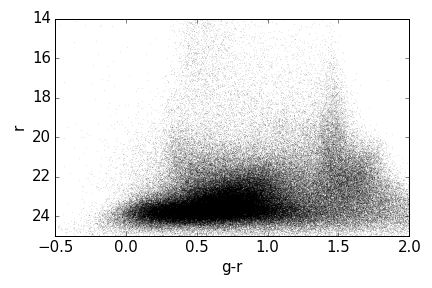
\includegraphics[width=\columnwidth]{Fig_2_Ivezic_2003_200000_sources.png}
 \caption{A color-magnitude plot, analogous to Figure 2 from Ivezi\'c+2003 . We use only 200 000 sources, corrected for galactic extinction,  plotting the median photometry over all epochs only for sources where median flux is not negative. }
\end{figure}

\section{Conclusions}
\label{sec:conclusions}



\section*{Acknowledgements}

Funding for the SDSS and SDSS-II has been provided by the Alfred P. Sloan Foundation, the Participating Institutions, the National Science Foundation, the U.S. Department of Energy, the National Aeronautics and Space Administration, the Japanese Monbukagakusho, the Max Planck Society, and the Higher Education Funding Council for England. The SDSS Web Site is http://www.sdss.org/.

The SDSS is managed by the Astrophysical Research Consortium for the Participating Institutions. The Participating Institutions are the American Museum of Natural History, Astrophysical Institute Potsdam, University of Basel, University of Cambridge, Case Western Reserve University, University of Chicago, Drexel University, Fermilab, the Institute for Advanced Study, the Japan Participation Group, Johns Hopkins University, the Joint Institute for Nuclear Astrophysics, the Kavli Institute for Particle Astrophysics and Cosmology, the Korean Scientist Group, the Chinese Academy of Sciences (LAMOST), Los Alamos National Laboratory, the Max-Planck-Institute for Astronomy (MPIA), the Max-Planck-Institute for Astrophysics (MPA), New Mexico State University, Ohio State University, University of Pittsburgh, University of Portsmouth, Princeton University, the United States Naval Observatory, and the University of Washington. 


%%%%%%%%%%%%%%%%%%%%%%%%%%%%%%%%%%%%%%%%%%%%%%%%%%

%%%%%%%%%%%%%%%%%%%% REFERENCES %%%%%%%%%%%%%%%%%%

% The best way to enter references is to use BibTeX:

%\bibliographystyle{mnras}
%\bibliography{example} % if your bibtex file is called example.bib

%%%%%%%%%%%%%%%%%%%%%%%%%%%%%%%%%%%%%%%%%%%%%%%%%%


% Don't change these lines
\bsp	% typesetting comment
\label{lastpage}
\end{document}

% End of mnras_template.tex
